We start our investigation by determining the work output $W$ when varying the time between qubit switching $\Delta \mathrm{T}$.
If the System qubit is initialised in the pure state $\rho_S = \ket{0} \bra{0}$, the work output for a single jump is given by (see appendix \ref{deriv_jump} for a derivation)
\begin{equation} \label{single_work}
	W = \frac{1}{\abs{\alpha}} \sin(2\abs{\alpha}\Delta \mathrm{T}) \Im{(\tau' - \tau) \alpha^*}
\end{equation}
\begin{equation*}
	\alpha = \frac{1}{2} \left[\sin(\theta_D^1) e^{i\phi_D^1} + \sin(\theta_T^1) e^{i\phi_T^1}\right], \\
	\tau' - \tau = \frac{1}{2} \left[ \sin(\theta_T^2)e^{i\phi_T^2} - \sin(\theta_T^1)e^{i\phi_T^1} \right].
\end{equation*}

We note that for $\Delta \mathrm{T} \to 0, W \to 0$. We simulate 500 random Drive functions for multiple values of $N$ and each $\Delta \mathrm{T}$, finding their optimal Transducer policy. The average work output over the 500 runs scaled by the amount of PWC steps $\overline{W}/N$ for 20 values of $\Delta \mathrm{T}$ is shown in figure \ref{dt_0}.

In \ref{dt_eigen}, we plot the average work when the system qubit is initialised in an eigenstate of partial system Hamiltonian acting only between drive and system $H_{DS} = \bra{\psi_D}\bra{\psi_T} H_I \otimes \mathds{1}_T \ket{\psi_D} \ket{\psi_T}$, $\rho_0 = \ket{+}\bra{+}$.
For $\Delta \mathrm{T} = 0$, the work output is $W = 1$ for all $N$. This is the amount of work that can be extracted by switching the Hamiltonian in such a way that the eigenvalues change signs.
A special case occurs for $N = 2$: the optimal case is independent of $\Delta \mathrm{T}$.
Here, the maximum work output per step of $W = 1$ can be achieved by setting the transducer such that the total system Hamiltonian commutes with $H_{DS}$. $\rho_S$ remains in the eigenstate and after time $\Delta \mathrm{T}$, \ $W = 1$ can be extracted from the system as with $\Delta \mathrm{T} = 0$.


\begin{figure}
	\centering
	\begin{subfigure}{0.4\textwidth}
		\centering
		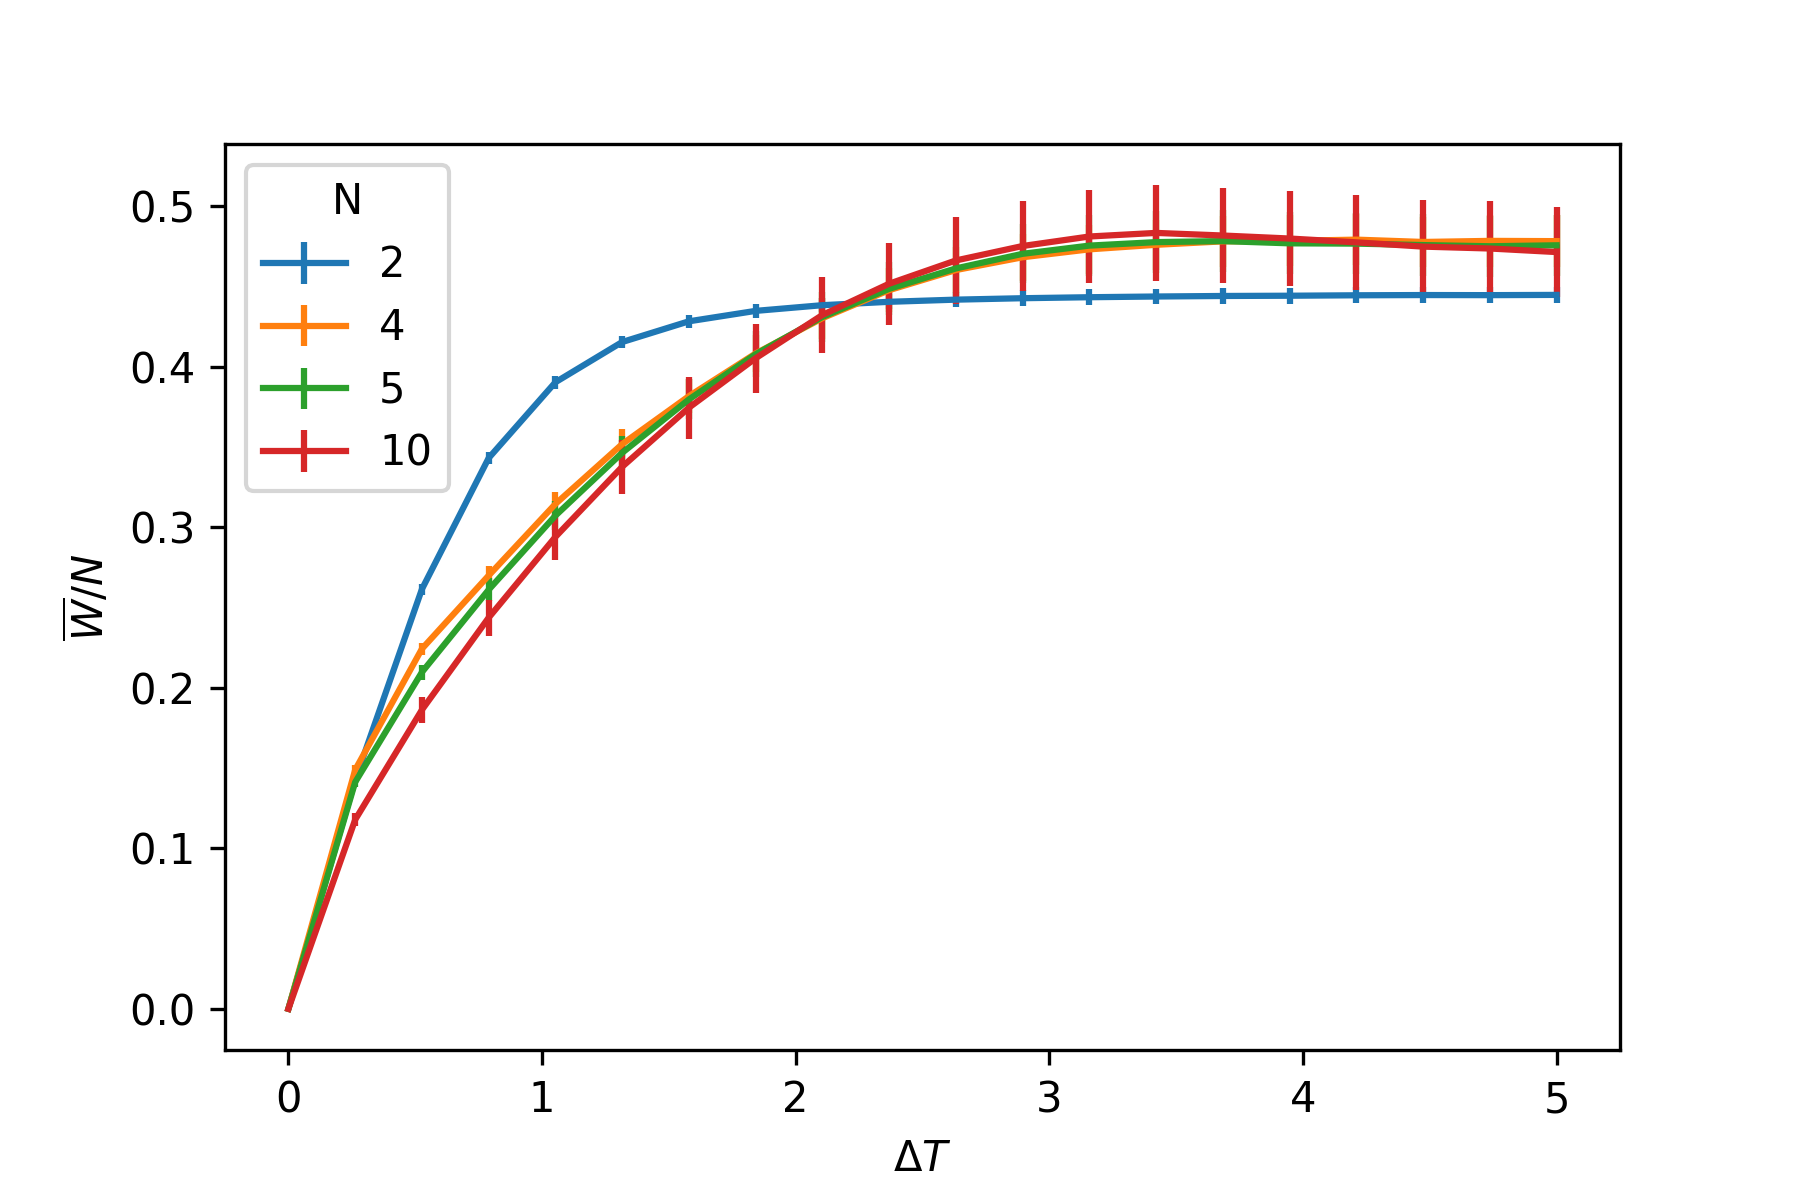
\includegraphics[width=\textwidth]{img/dt_0}
		\caption{$\rho_0 = \ket{0}\bra{0}$}
		\label{dt_0}
	\end{subfigure}
	\begin{subfigure}{0.4\textwidth}
	\centering
	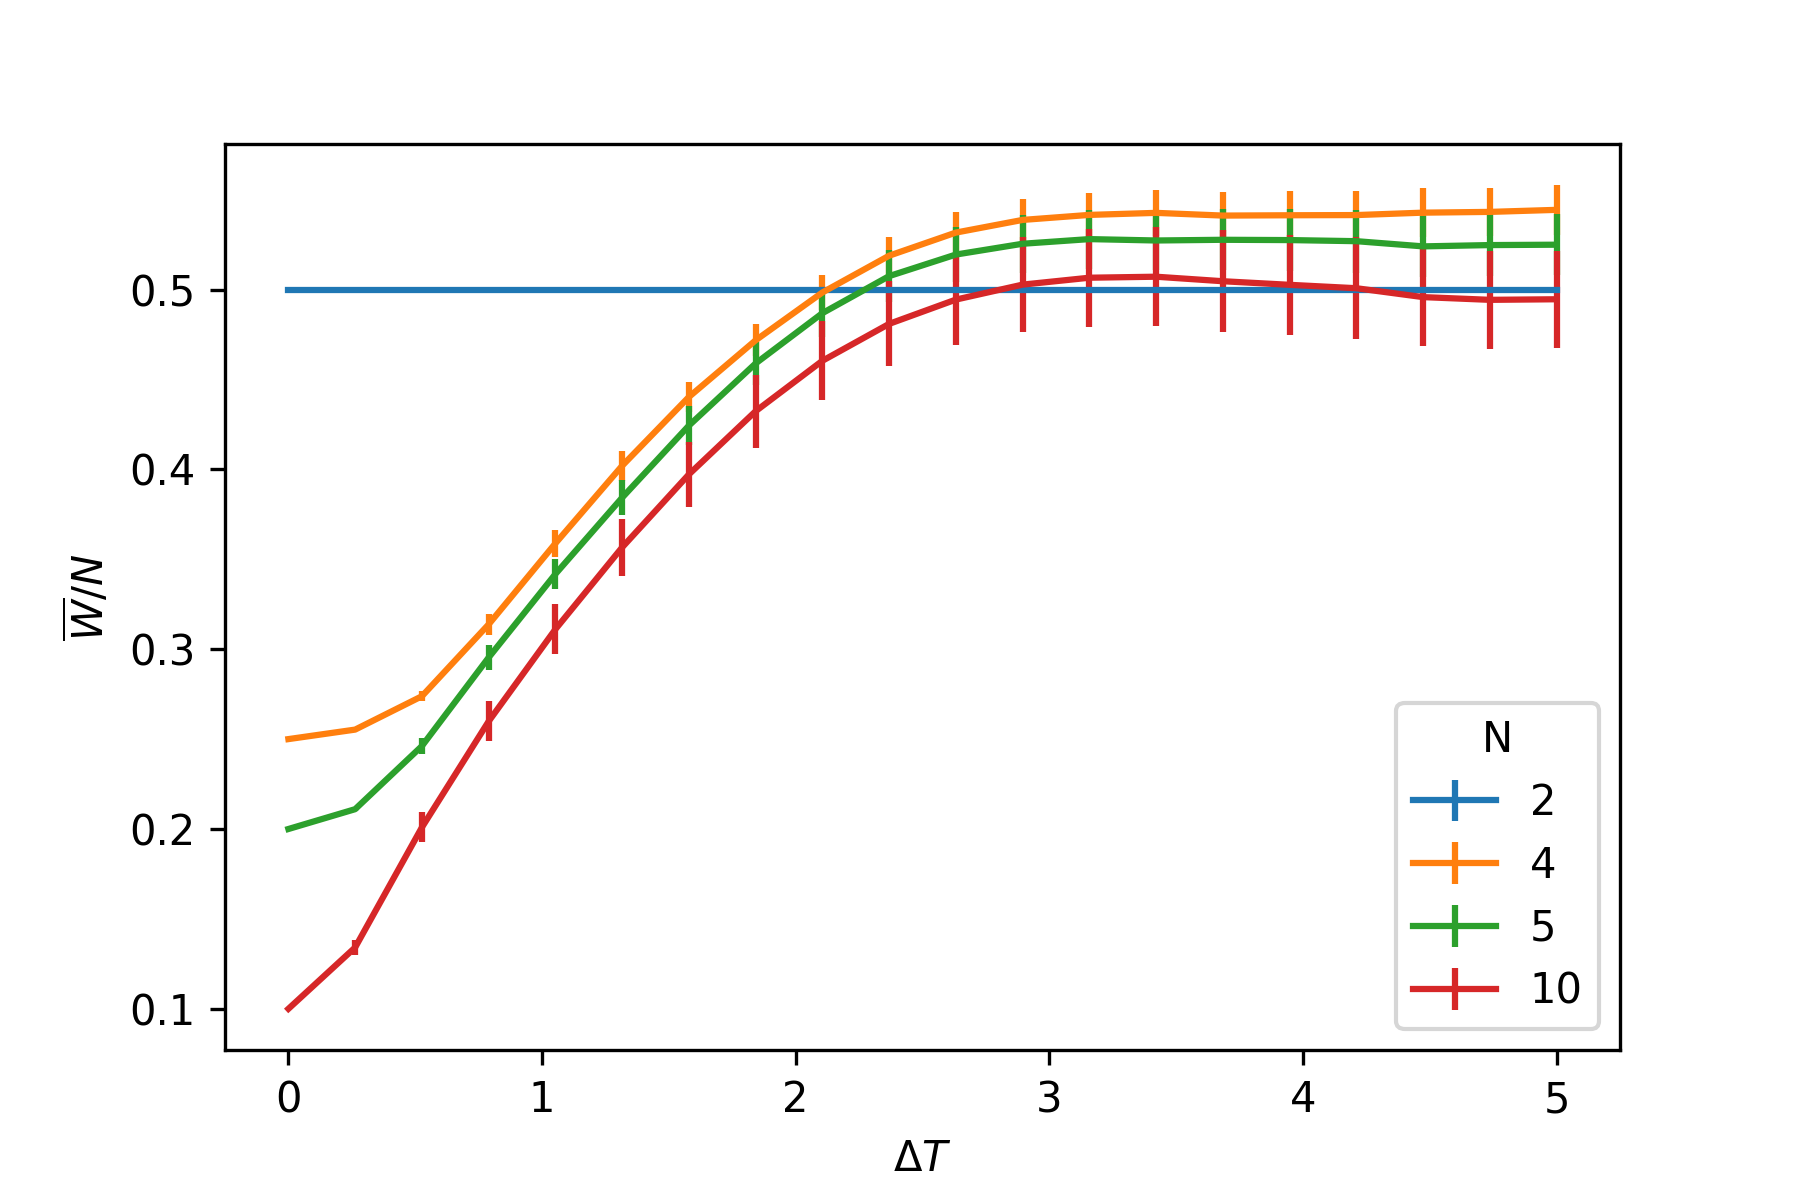
\includegraphics[width=\textwidth]{img/dt_eigen}
	\caption{$\rho_0 = \ket{+}\bra{+}$}
	\label{dt_eigen}
	\end{subfigure}
	\caption{(a) We plot the average work $\overline{W}$ over 500 runs of random excitations divided by amount of PWC steps $N$, with $\rho_0 = \ket{0}\bra{0}$, for multiple $N$. The error bars correspond to the standard deviation $\sigma_{\overline{W}}$.
	(b) We plot $\overline{W}/N$ for multiple $N$ where the system state is initialised in an eigenstate of the Drive Hamiltonian $H_{DS}$.}
	\label{dt_dep}
\end{figure}